\documentclass[10pt, a4paper]{article}
% \usepackage[english]{babel}
\usepackage[brazilian]{babel}
\usepackage[utf8]{inputenc}
% \usepackage[T1]{fontenc}
\usepackage{lipsum}

% code
\usepackage{pythonhighlight}
\renewcommand{\lstlistingname}{Anexo} % Listing->Code
\usepackage{adjustbox}

% For subfigure use
\usepackage[font=small,labelfont=bf]{caption}
\usepackage{subcaption}

% Set page size and margins
% Replace `letterpaper' with`a4paper' for UK/EU standard size
\usepackage[a4paper,top=2cm,bottom=2cm,left=2cm,right=2cm,marginparwidth=2cm]{geometry}

% tabelas
\usepackage{array}
\usepackage{tabularx}
\usepackage{booktabs}

\usepackage{float}

% Useful packages
\usepackage{amsmath}
\usepackage{enumerate}

\usepackage{graphicx}
\usepackage[colorlinks=true, allcolors=blue]{hyperref}
\usepackage{cleveref}
%\usepackage[notransparent]{svg}
\newcommand{\crefrangeconjunction}{--}


\begin{document}

\def\TITLE{Trabalho 01}
\def\DISCIPLINE{MEC 2403 - Otimização e Algoritmos para Engenharia Mecânica}
\def\PROFESSOR{Ivan Menezes}
\def\AUTHOR{Pedro Henrique Cardoso Paulo}
\def\CONTACT{pedrorjpaulo.phcp@gmail.com}
\def\DATE{maio de 2023}

\title{\textbf{\TITLE} \\ \DISCIPLINE}
\author{\AUTHOR}
\date{\DATE}

\begin{titlepage}
      \begin{center}
          \vspace*{1cm}

          \Huge
          \textbf{\TITLE}

          \vspace{0.5cm}
          \LARGE
          \DISCIPLINE

          \vspace{1.5cm}

          \textbf{\AUTHOR \\ {\tt \CONTACT}}

          \vfill
          Professor: \PROFESSOR

          \vspace{0.8cm}

          
\includegraphics[width=0.2\textwidth]{../general/puc.jpg}

          \Large
          Departamento de Engenharia Mecânica\\
          PUC-RJ Pontifícia Universidade Católica do Rio de Janeiro\\
          \DATE

      \end{center}
  \end{titlepage}

\maketitle

\section{Introdução}

\subsection{Objetivos}

Esse é o entregável da \TITLE \ da disciplina \DISCIPLINE. Esse trabalho tem como objetivos:

\begin{enumerate}
  \item Aplicar os principais métodos de otimização sem restrição (OSR) implementados na \href{https://github.com/prj-phcp/MEC2403_Activities/blob/master/Lista2/Lista2.pdf}{Lista 02}
  \item Comparar os valores obtidos e número de passos para funções quadráticas e não quadráticas com o previsto pela literatura para cada método
  \item Aplicar os otimizadores em problemas complexos e testar sua escalabilidade
\end{enumerate}

\subsection{Links úteis}\label{links}

Nesta seção são listados alguns links e referências úteis para se entender o trabalho desempenhado.

\begin{enumerate}
  \item \href{https://web.tecgraf.puc-rio.br/~ivan/MEC2403/ProgMatematica_VazPereiraMenezes-Ago2012.pdf}{Apostila de programação matemática da disciplina}
  \item \href{https://github.com/prj-phcp/MEC2403_Activities}{GitHub usado para essa disciplina}
  \item \href{https://github.com/prj-phcp/MEC2403_Activities/blob/master/Trabalho1/Trabalho1.ipynb}{Notebook com o código para as figuras desse relatório}
  \item \href{https://github.com/prj-phcp/MEC2403_Activities/blob/master/Trabalho1/Derivadas.ipynb}{Notebook com o código para derivação simbólica das funções mais complexas}
  \item \href{https://github.com/prj-phcp/MEC2403_Activities/blob/master/packages}{Pasta com os códigos a serem aproveitados em todas as listas}
\end{enumerate}

\section{Questão 01}\label{sec:q01}

\subsection{Enunciado}

Implementar, usando o MATLAB ou Python, os métodos de otimização: (a) \textit{Univariante}; (b) \textit{Powell}; (c) \textit{Steepest Descent}; 
(d) \textit{Fletcher–Reeves}; (e) \textit{BFGS}; e (f) \textit{Newton–Raphson}. Adotar o método da Seção Áurea para a realização das buscas unidirecionais
(line search). Para verificação da convergência numérica, utilizar uma tolerância de $10^{-5}$. Em seguida, testar a sua implementação encontrando os pontos
de mínimo das seguintes funções:

\begin{enumerate}[(a)]
  \item $f(x_1, x_2) = x_1^2 - 3x_1x_2 + 4x_2^2 + x_1 - x_2$ \\
        Pontos iniciais: $\mathbf{x^0} = [2, 2]^T$ e $\mathbf{x^0} = [-1, -3]^T$, \label{func:a}
  \item $f(x_1, x_2) = (1 + a - bx_1 - bx_2)^2 + (b + x_1 + ax_2 - bx_1x_2)^2, \ a = 10, \ b = 1$ \\
        Pontos iniciais: $\mathbf{x^0} = [10, 2]^T$ e $\mathbf{x^0} = [-2, -3]^T$, \label{func:b}
\end{enumerate}

\subsection{Solução}

\begin{figure}[htpb]
  \centering
  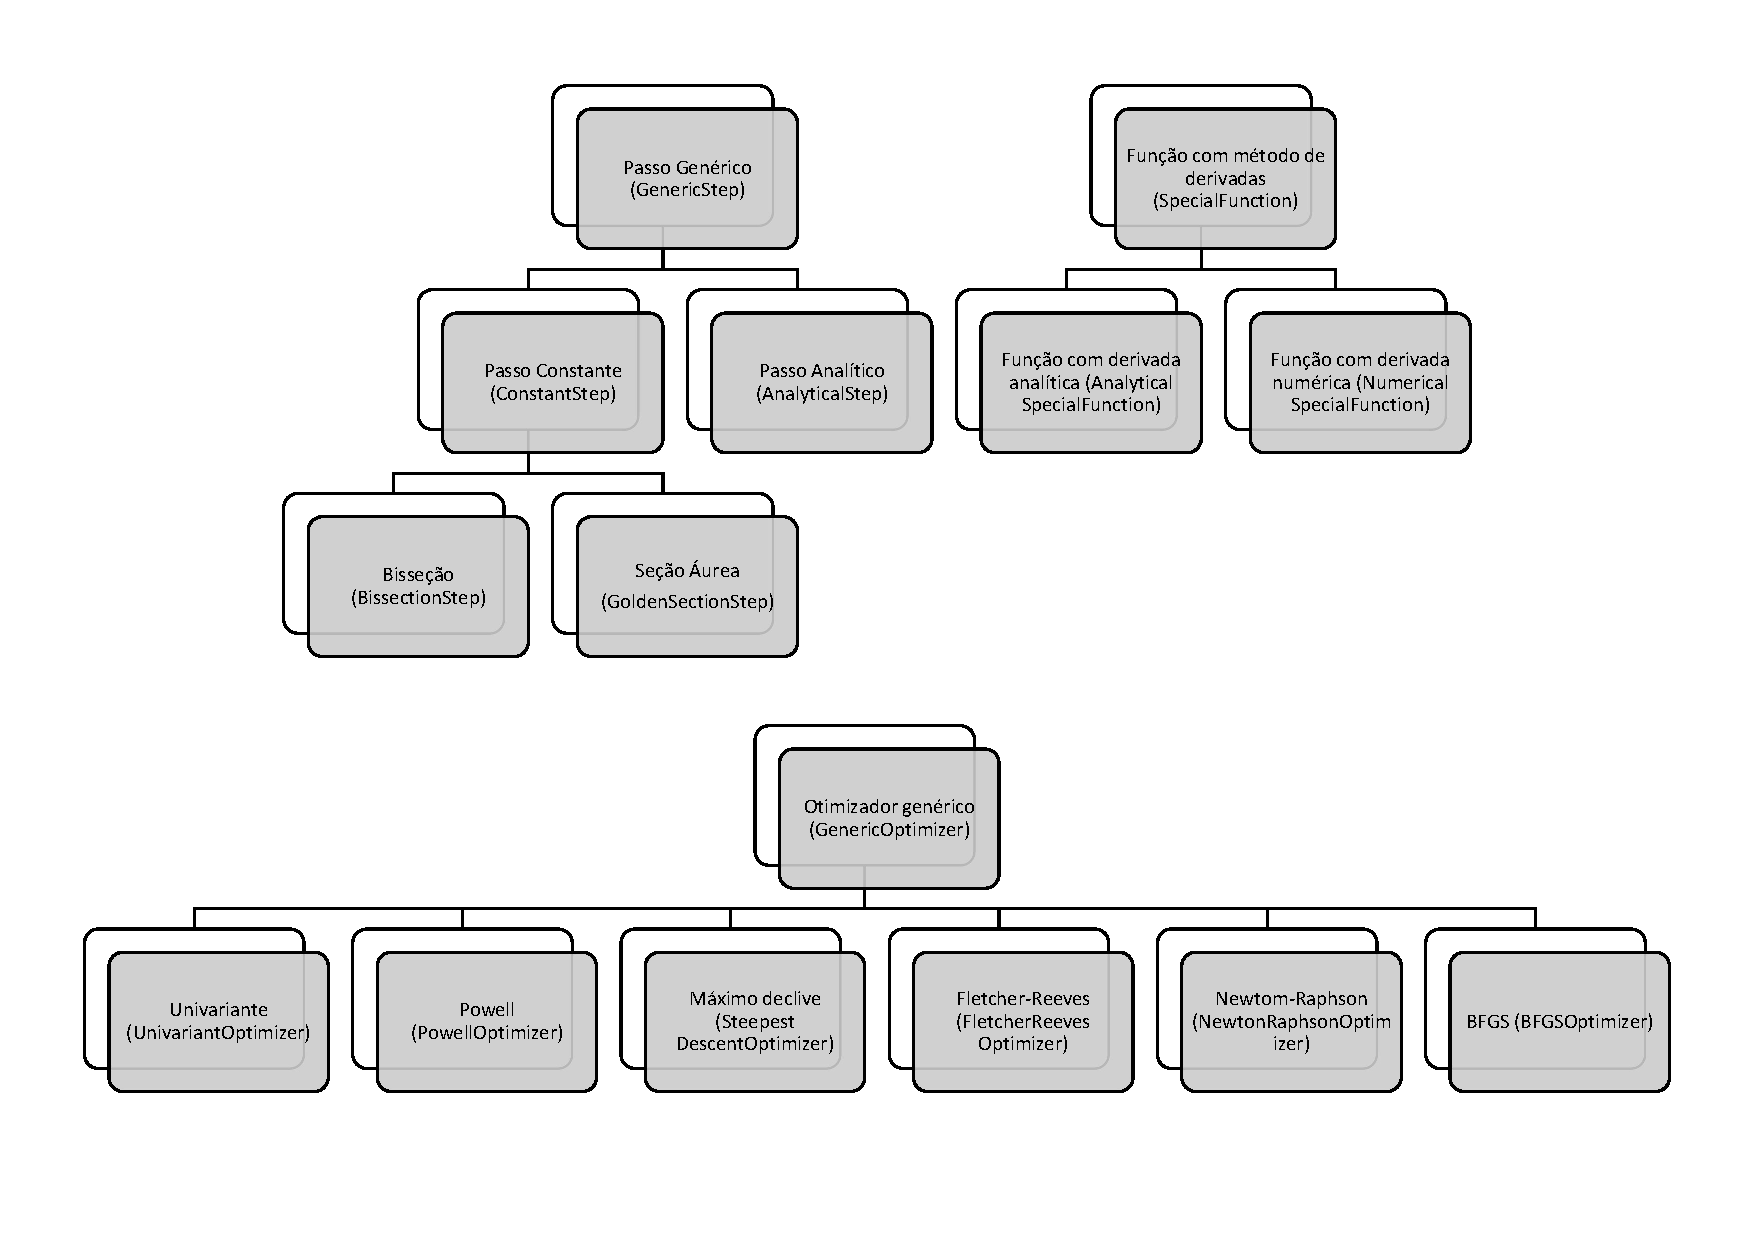
\includegraphics[width=0.8\textwidth]{../general/classes_full.pdf}
  \caption{Estrutura de classes implementada e heranças}
  \label{fig:q1_1}
\end{figure}

\subsubsection{Item \ref{func:a}}

\begin{table}[htpb]
  \centering
  \begin{tabular}{|l|c|c|c|c|c|}
    \cline{2-5}
    \multicolumn{1}{c}{} \vline
    & 
    \multicolumn{2}{c}{$\mathbf{x^0} = [2, 2]^T$} \vline
    & 
    \multicolumn{2}{c}{$\mathbf{x^0} = [-1, -3]^T$} \vline \\
    \hline%\cline{2-5}
    Método             &	Ponto de mínimo	          & Passos	&  Ponto de mínimo	          &  Passos   \\
    \hline
    Univariante        & $[-0.714275, -0.142853]^T$ & 46      &  $[-0.714293, -0.142860]^T$ &  48       \\
    Powell             & $[-0.714286, -0.142857]^T$ & 6       &  $[-0.714286, -0.142857]^T$ &  6        \\
    Steepest Descent   & $[-0.714280, -0.142855]^T$ & 32      &  $[-0.714294, -0.142861]^T$ &  7        \\
    Fletcher-Reeves    & $[-0.714286, -0.142857]^T$ & 2       &  $[-0.714286, -0.142858]^T$ &  2        \\
    Newton-Raphson     & $[-0.714286, -0.142857]^T$ & 1       &  $[-0.714286, -0.142857]^T$ &  1        \\
    BFGS               & $[-0.714286, -0.142857]^T$ & 2       &  $[-0.714286, -0.142857]^T$ &  2        \\
    \hline
  \end{tabular}
  \caption{Resumo dos resultados obtidos para a função (\ref{func:a})}
  \label{tab:q1a_results}
\end{table}

\begin{figure}[htpb]
  \centering
  \begin{subfigure}[b]{0.32\textwidth}
      \centering
      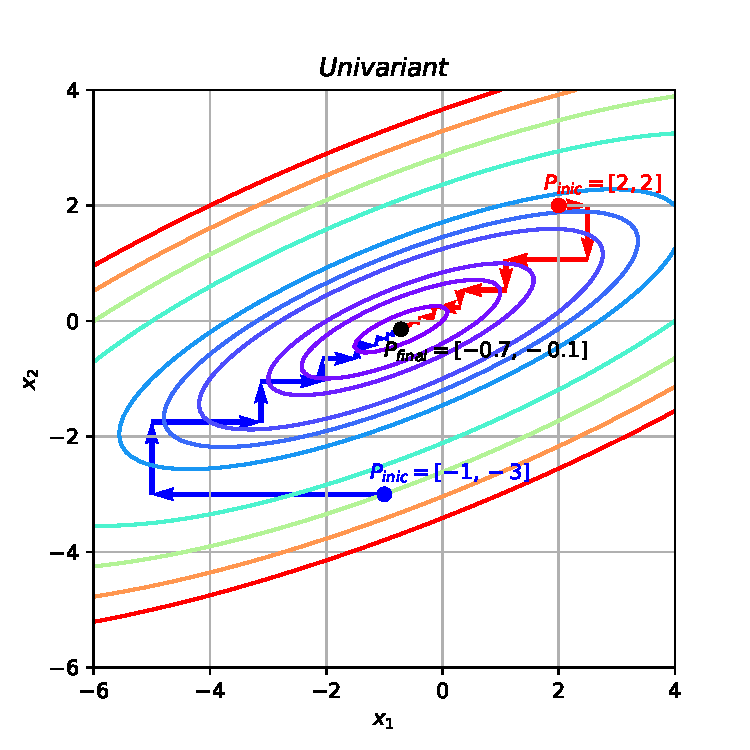
\includegraphics[width=\textwidth]{images/q1a_Univariant.pdf}
      \caption{Univariante}
      \label{fig:q1a_univariant}
  \end{subfigure}
  \hfill
  \begin{subfigure}[b]{0.32\textwidth}
    \centering
    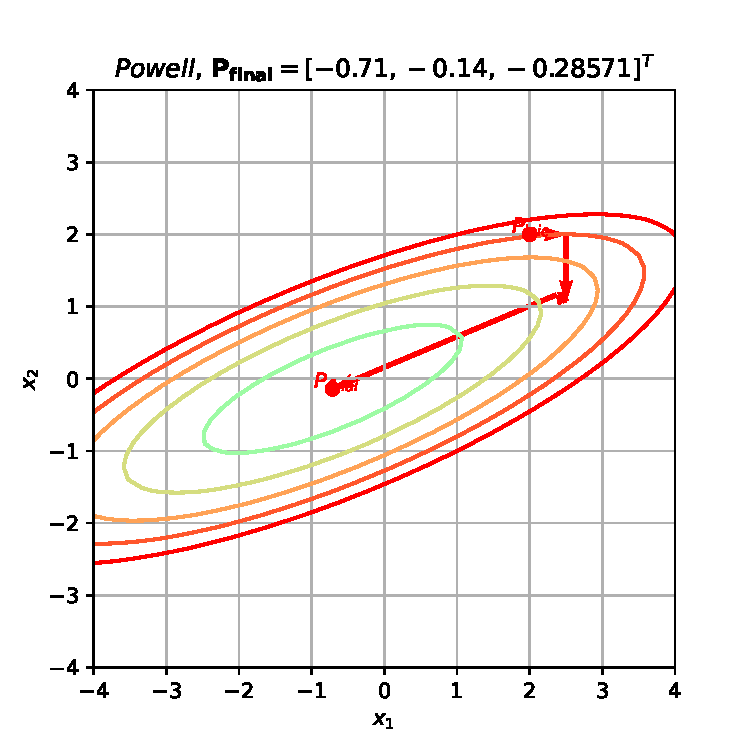
\includegraphics[width=\textwidth]{images/q1a_Powell.pdf}
    \caption{Powell}
    \label{fig:q1a_powell}
  \end{subfigure}
  \hfill
  \begin{subfigure}[b]{0.32\textwidth}
    \centering
    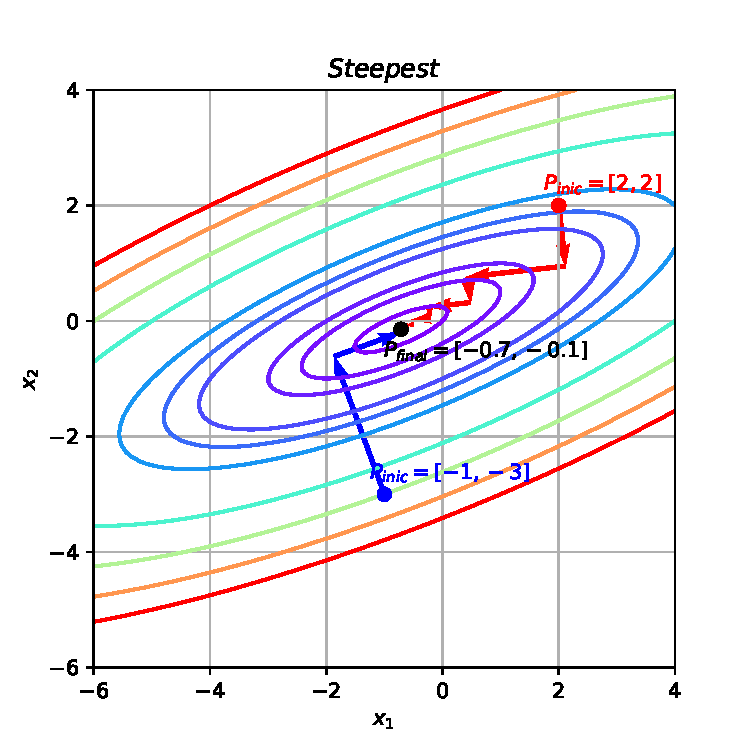
\includegraphics[width=\textwidth]{images/q1a_Steepest.pdf}
    \caption{Steepest Descent}
    \label{fig:q1a_steepest}
  \end{subfigure}
  \hfill
  \begin{subfigure}[b]{0.32\textwidth}
    \centering
    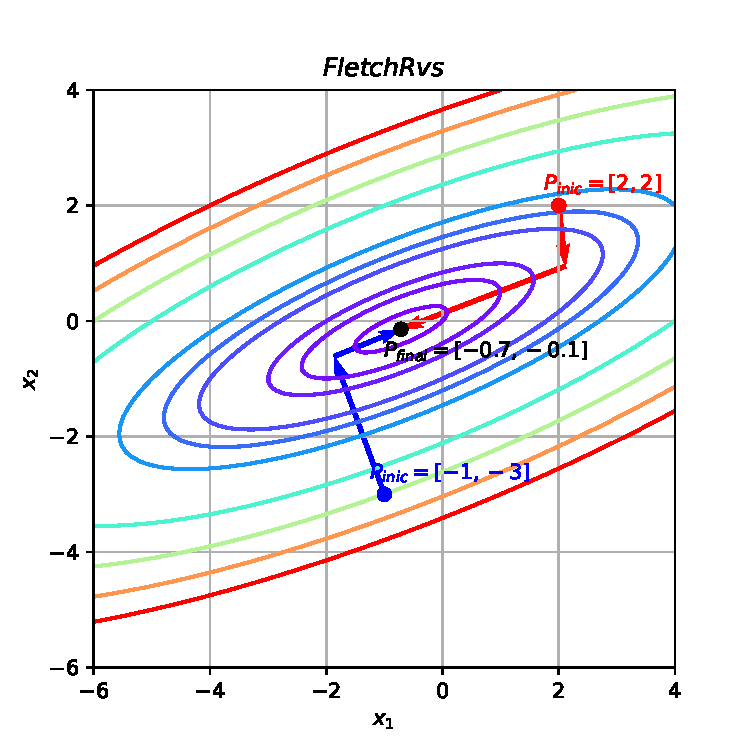
\includegraphics[width=\textwidth]{images/q1a_FletchRvs.pdf}
    \caption{Fletcher-Reeves}
    \label{fig:q1a_fletchrvs}
  \end{subfigure}
  \hfill
  \begin{subfigure}[b]{0.32\textwidth}
    \centering
    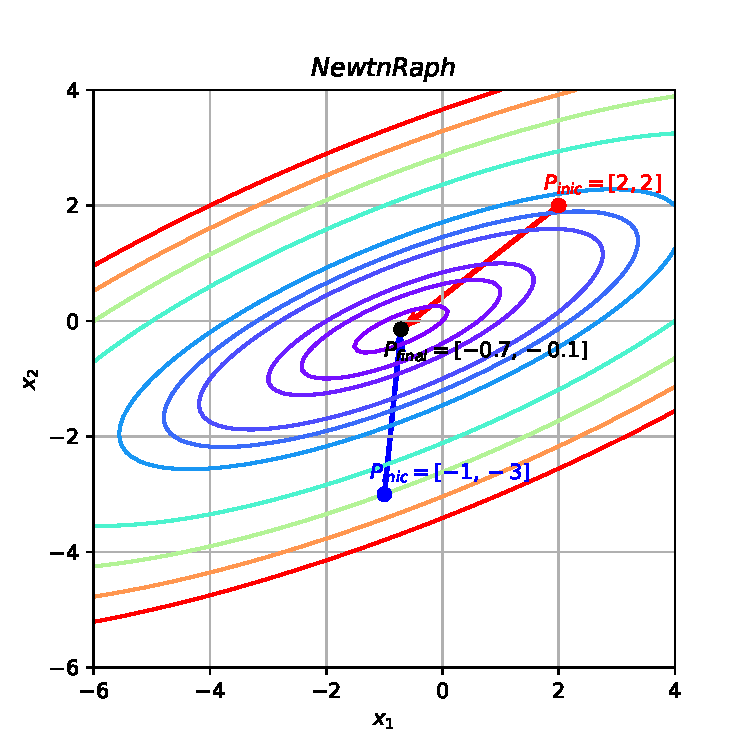
\includegraphics[width=\textwidth]{images/q1a_NewtnRaph.pdf}
    \caption{Newton-Raphson}
    \label{fig:q1a_newtnraph}
  \end{subfigure}
  \hfill
  \begin{subfigure}[b]{0.32\textwidth}
    \centering
    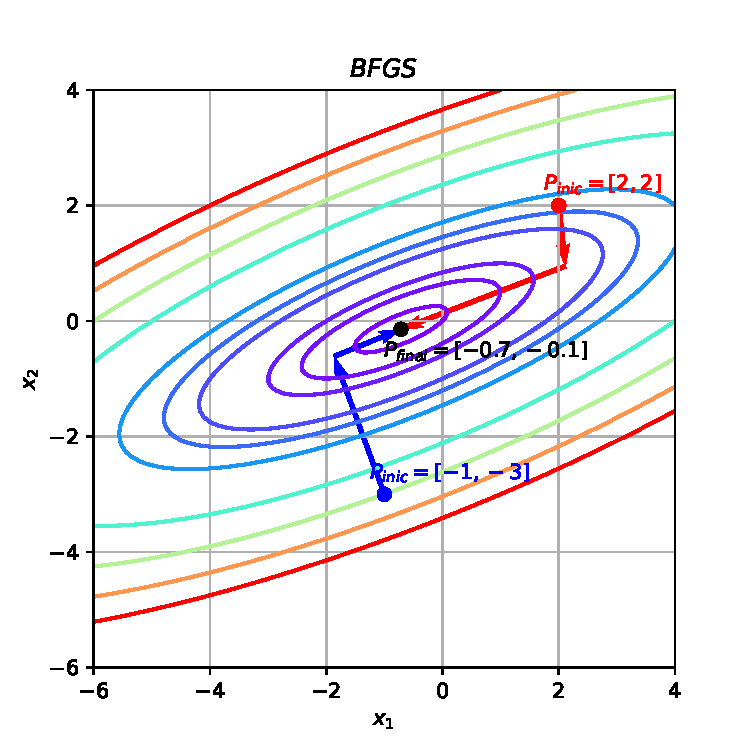
\includegraphics[width=\textwidth]{images/q1a_BFGS.pdf}
    \caption{BFGS}
    \label{fig:q1a_bfgs}
  \end{subfigure}
     \caption{Resultados gráficos para a função \ref{func:a}}
     \label{fig:q1a}
\end{figure}

\subsubsection{Item \ref{func:b}}

\begin{figure}[htpb]
  \centering
  \begin{subfigure}[b]{0.32\textwidth}
      \centering
      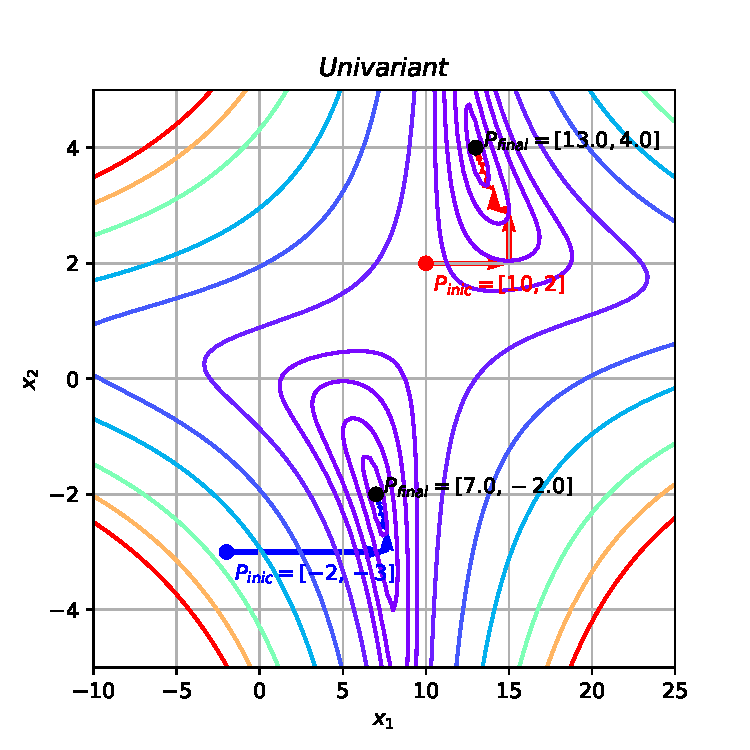
\includegraphics[width=\textwidth]{images/q1b_Univariant.pdf}
      \caption{Univariante}
      \label{fig:q1b_univariant}
  \end{subfigure}
  \hfill
  \begin{subfigure}[b]{0.32\textwidth}
    \centering
    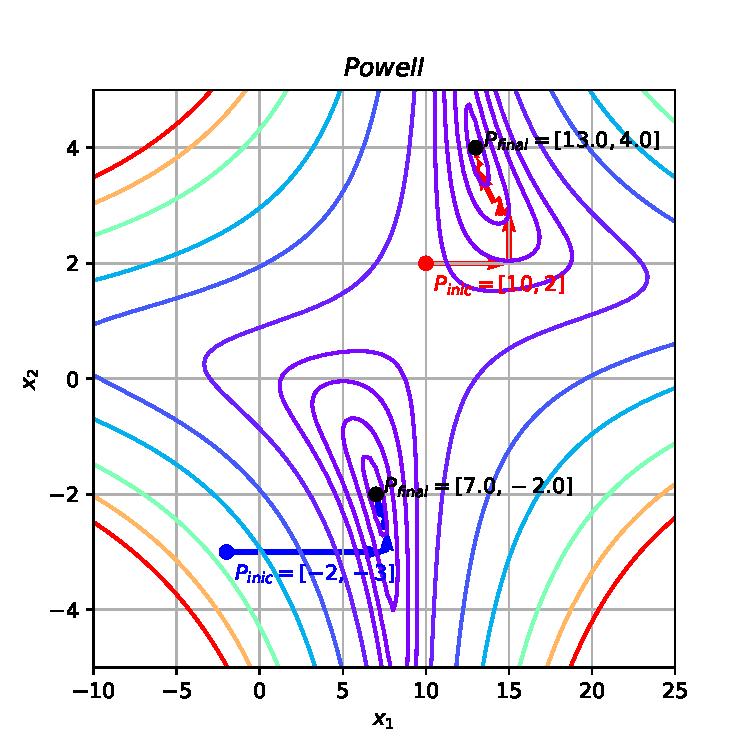
\includegraphics[width=\textwidth]{images/q1b_Powell.pdf}
    \caption{Powell}
    \label{fig:q1b_powell}
  \end{subfigure}
  \hfill
  \begin{subfigure}[b]{0.32\textwidth}
    \centering
    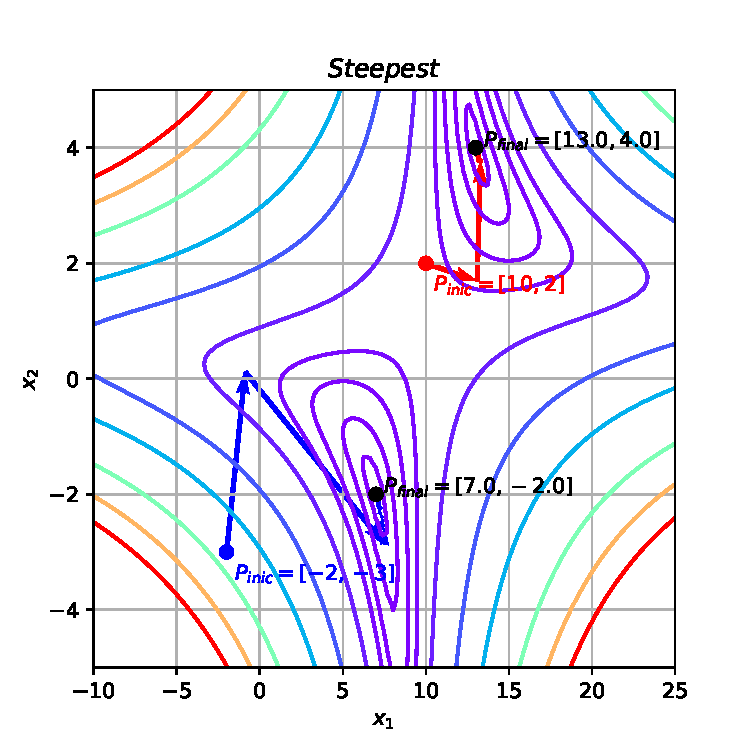
\includegraphics[width=\textwidth]{images/q1b_Steepest.pdf}
    \caption{Steepest Descent}
    \label{fig:q1b_steepest}
  \end{subfigure}
  \hfill
  \begin{subfigure}[b]{0.32\textwidth}
    \centering
    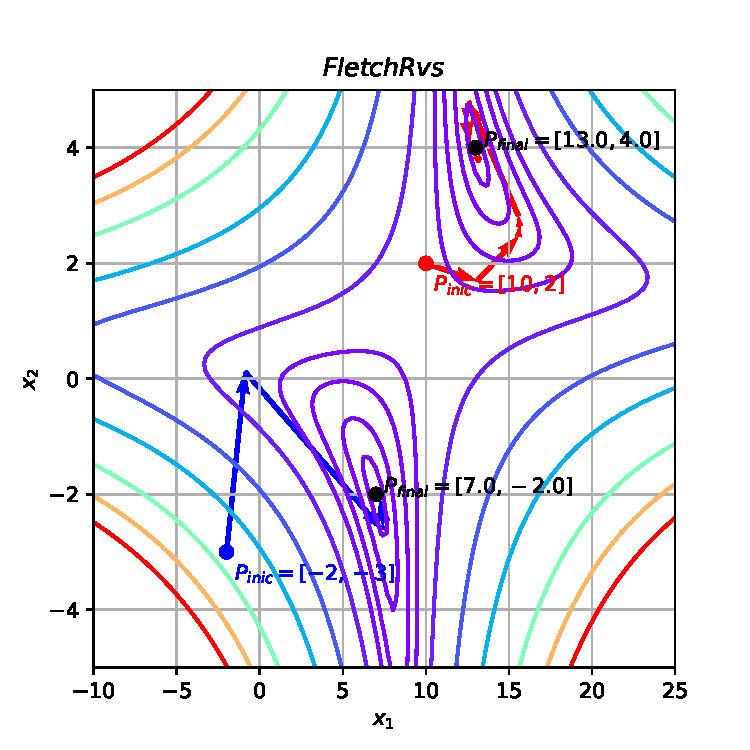
\includegraphics[width=\textwidth]{images/q1b_FletchRvs.pdf}
    \caption{Fletcher-Reeves}
    \label{fig:q1b_fletchrvs}
  \end{subfigure}
  \hfill
  \begin{subfigure}[b]{0.32\textwidth}
    \centering
    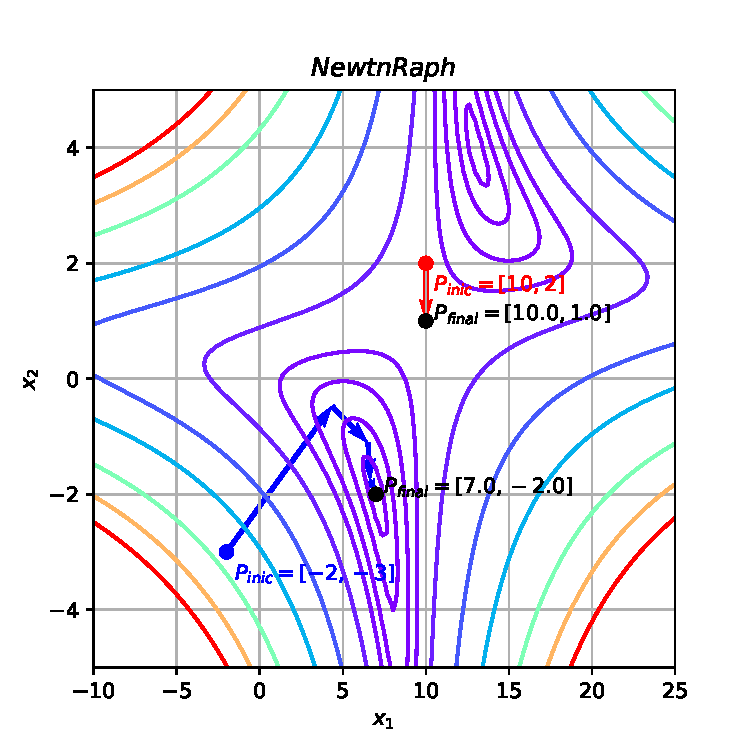
\includegraphics[width=\textwidth]{images/q1b_NewtnRaph.pdf}
    \caption{Newton-Raphson}
    \label{fig:q1b_newtnraph}
  \end{subfigure}
  \hfill
  \begin{subfigure}[b]{0.32\textwidth}
    \centering
    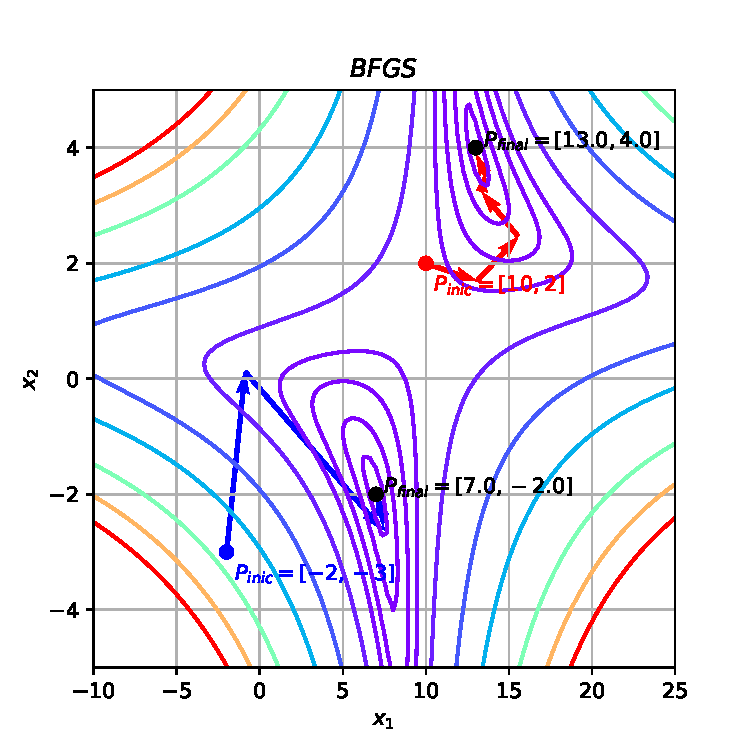
\includegraphics[width=\textwidth]{images/q1b_BFGS.pdf}
    \caption{BFGS}
    \label{fig:q1b_bfgs}
  \end{subfigure}
     \caption{Resultados gráficos para a função \ref{func:b}}
     \label{fig:q1b}
\end{figure}

\section{Questão 02}

\subsection{Enunciado}

Utilizando os métodos de otimização implementados na primeira questão:

\begin{enumerate}[(a)]
  \item Determinar os deslocamentos $(u_A, v_A)$, do ponto $A$, que minimizam a Energia Potencial Total $\Pi$ do sistema de molas indicado na figura abaixo. \
  Adotar o ponto inicial: $x_0 = [0.01, -0.10]^T$.
  \item desenvolver um estudo de convergência da solução deste problema (i.e., deslocamento do ponto $A$) para níveis crescentes de discretização \
  do modelo (ou seja, considerando o número de molas $n = 2, 4, 6, ...$ ). Se possível, comparar as suas respostas com as soluções obtidas usando o Método \
  dos Elementos Finitos (levando em consideração o comportamento não linear geométrico da estrutura). A rigidez de cada mola ($k_i = 1, ..., n$) é obtida como a \
  razão entre o módulo de rigidez axial do material e o seu comprimento. Os valores $W_j$ (com $j = 1, ..., n$) correspondem às cargas nodais equivalentes aos pesos \
  das molas.
\end{enumerate}

\subsection{Solução}

\subsubsection{Determinação do mínimo}

\begin{figure}[htpb]
  \centering
  \begin{subfigure}[b]{0.32\textwidth}
      \centering
      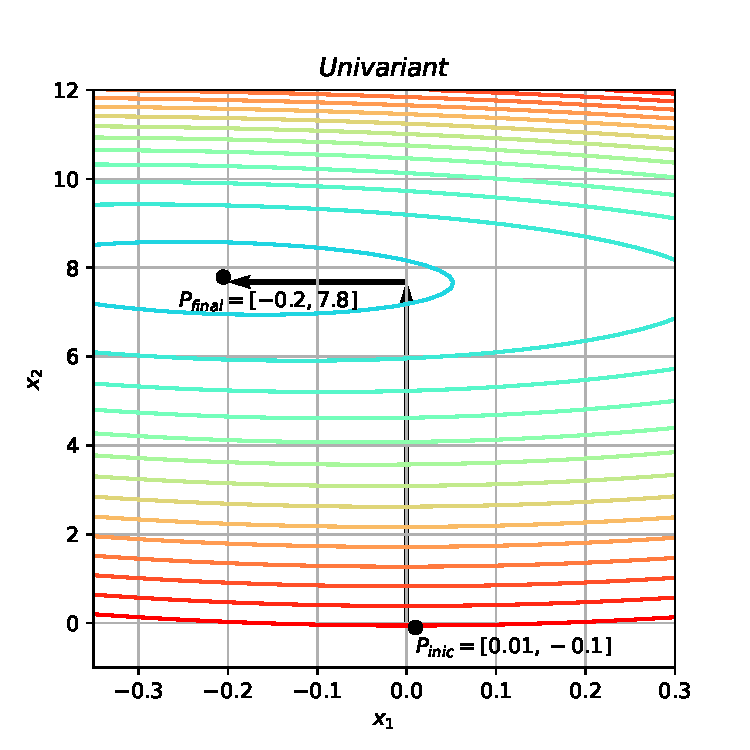
\includegraphics[width=\textwidth]{images/q2a_Univariant.pdf}
      \caption{Univariante}
      \label{fig:q2a_univariant}
  \end{subfigure}
  \hfill
  \begin{subfigure}[b]{0.32\textwidth}
    \centering
    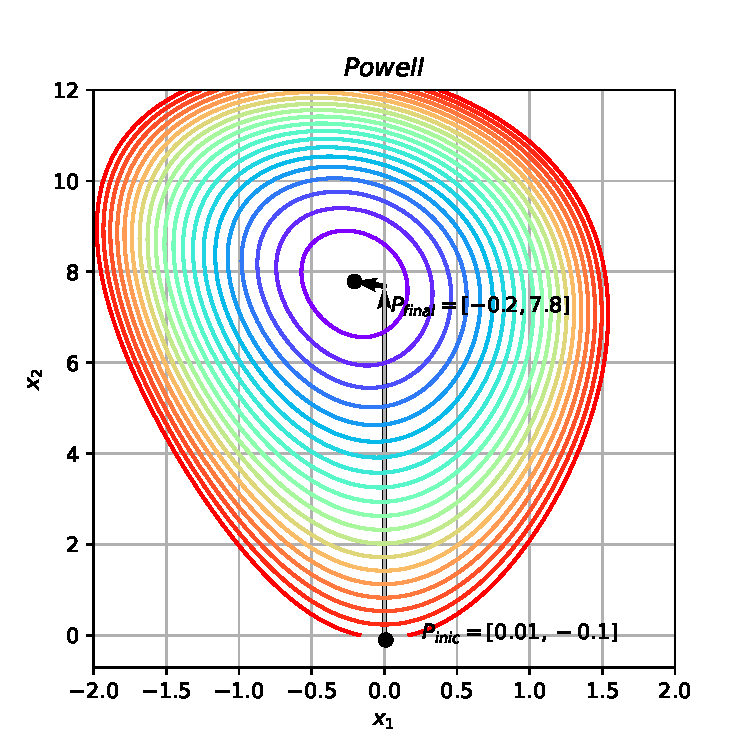
\includegraphics[width=\textwidth]{images/q2a_Powell.pdf}
    \caption{Powell}
    \label{fig:q2a_powell}
  \end{subfigure}
  \hfill
  \begin{subfigure}[b]{0.32\textwidth}
    \centering
    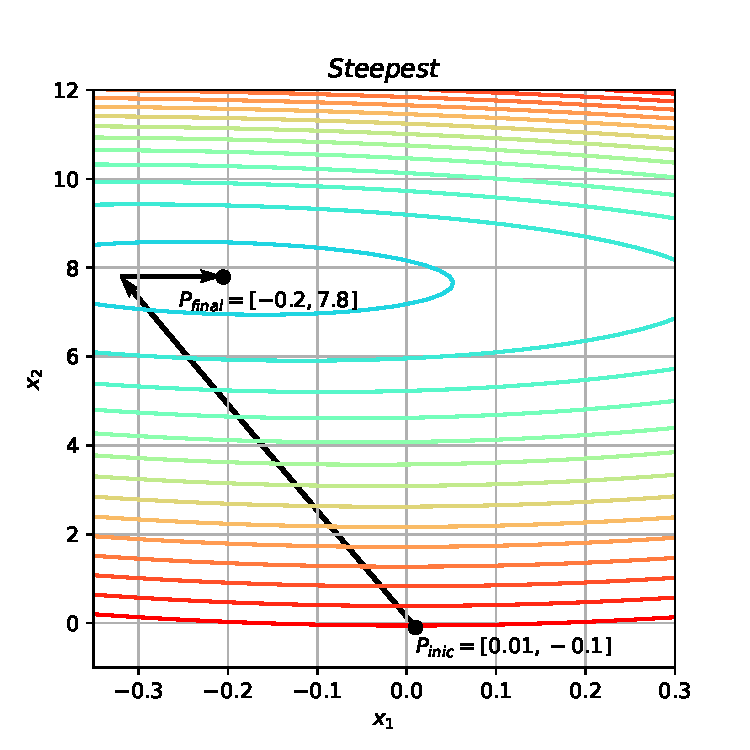
\includegraphics[width=\textwidth]{images/q2a_Steepest.pdf}
    \caption{Steepest Descent}
    \label{fig:q2a_steepest}
  \end{subfigure}
  \hfill
  \begin{subfigure}[b]{0.32\textwidth}
    \centering
    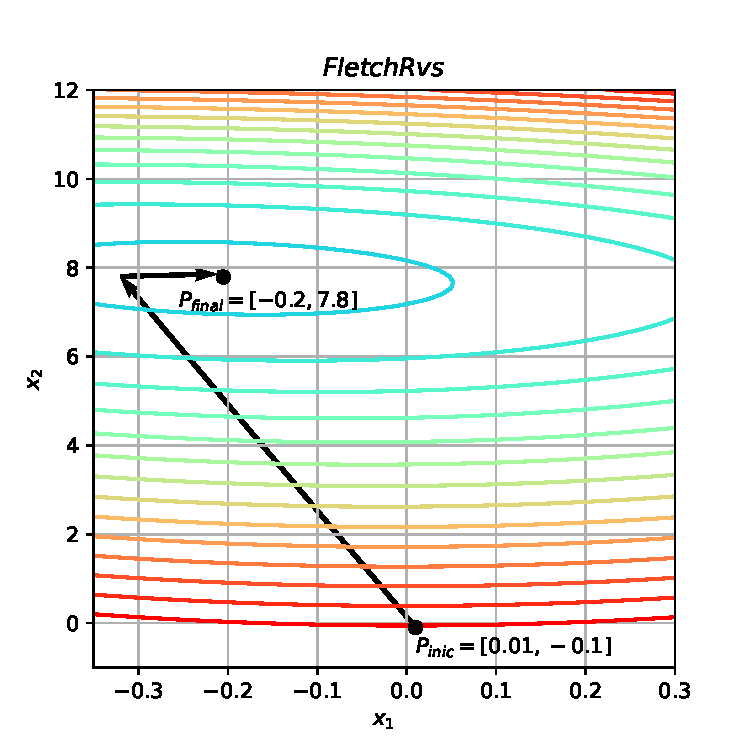
\includegraphics[width=\textwidth]{images/q2a_FletchRvs.pdf}
    \caption{Fletcher-Reeves}
    \label{fig:q2a_fletchrvs}
  \end{subfigure}
  \hfill
  \begin{subfigure}[b]{0.32\textwidth}
    \centering
    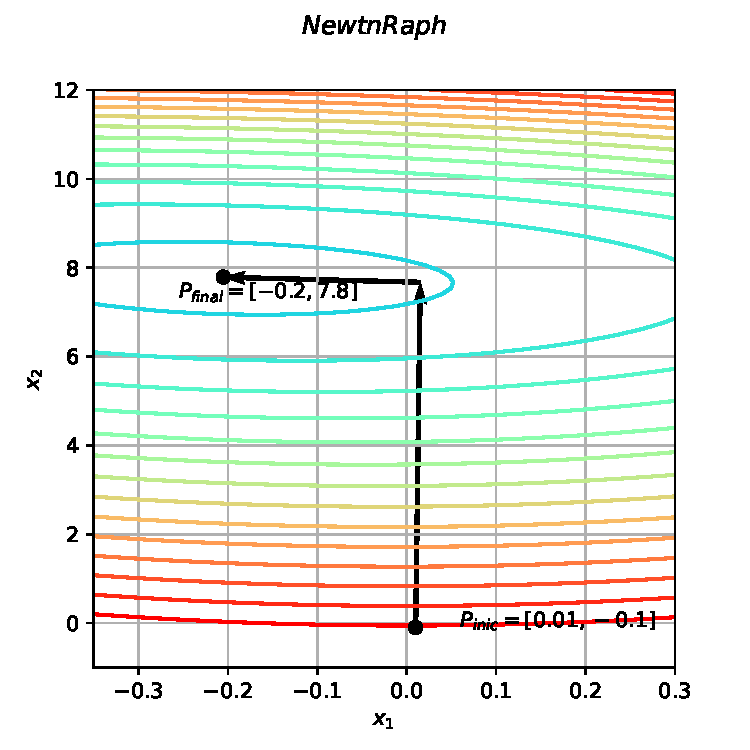
\includegraphics[width=\textwidth]{images/q2a_NewtnRaph.pdf}
    \caption{Newton-Raphson}
    \label{fig:q2a_newtnraph}
  \end{subfigure}
  \hfill
  \begin{subfigure}[b]{0.32\textwidth}
    \centering
    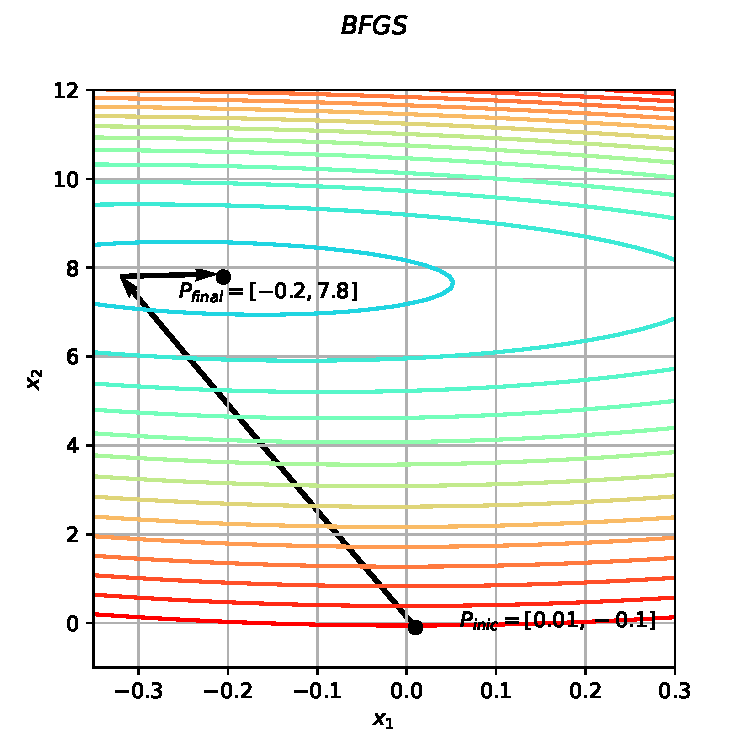
\includegraphics[width=\textwidth]{images/q2a_BFGS.pdf}
    \caption{BFGS}
    \label{fig:q2a_bfgs}
  \end{subfigure}
     \caption{Resultados gráficos da determinação do mínimo da função potencial}
     \label{fig:q2a}
\end{figure}

\subsubsection{Análise de convergência}

\begin{figure}[htpb]
  \centering
  \begin{subfigure}[b]{0.32\textwidth}
      \centering
      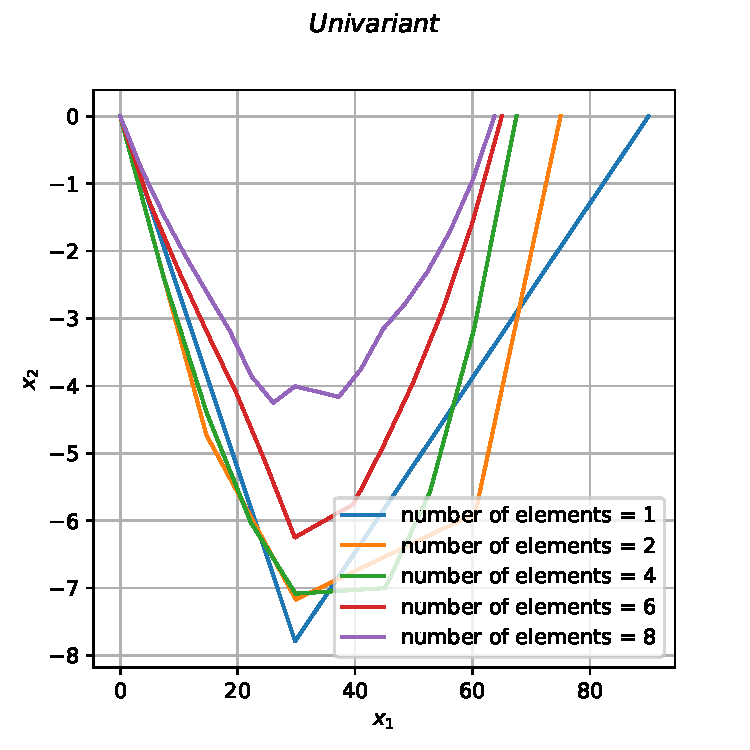
\includegraphics[width=\textwidth]{images/q2b_Univariant.pdf}
      \caption{Univariante}
      \label{fig:q2b_univariant}
  \end{subfigure}
  \hfill
  \begin{subfigure}[b]{0.32\textwidth}
    \centering
    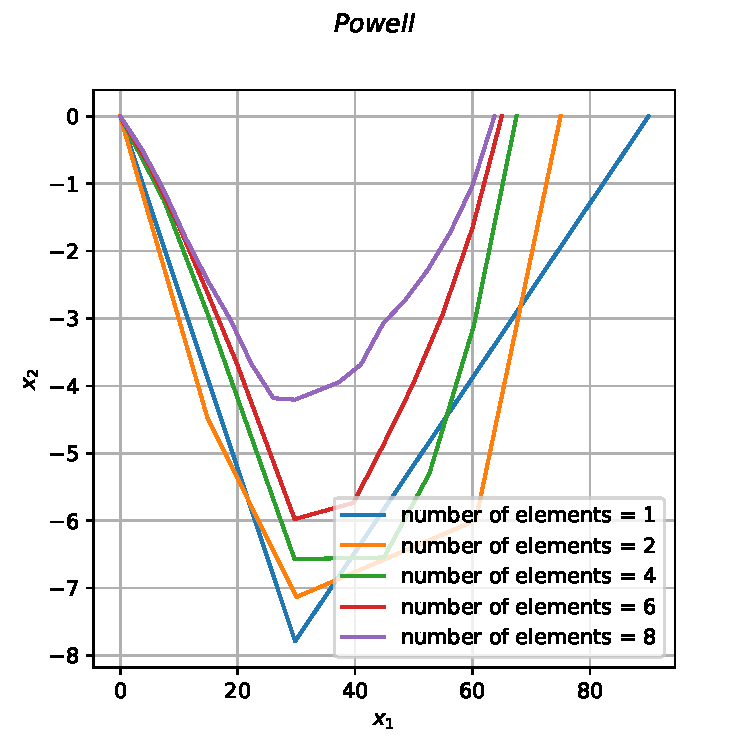
\includegraphics[width=\textwidth]{images/q2b_Powell.pdf}
    \caption{Powell}
    \label{fig:q2b_powell}
  \end{subfigure}
  \hfill
  \begin{subfigure}[b]{0.32\textwidth}
    \centering
    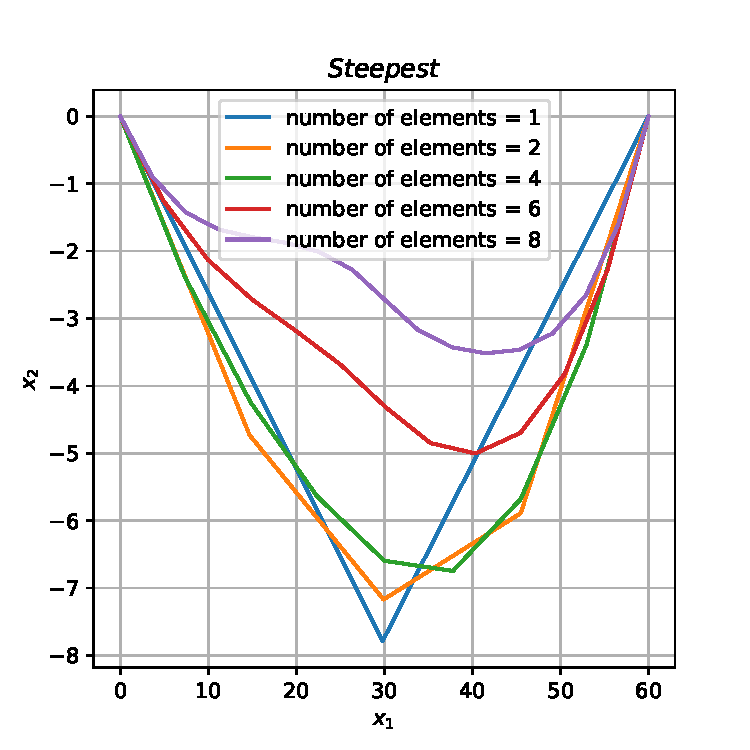
\includegraphics[width=\textwidth]{images/q2b_Steepest.pdf}
    \caption{Steepest Descent}
    \label{fig:q2b_steepest}
  \end{subfigure}
  \hfill
  \begin{subfigure}[b]{0.32\textwidth}
    \centering
    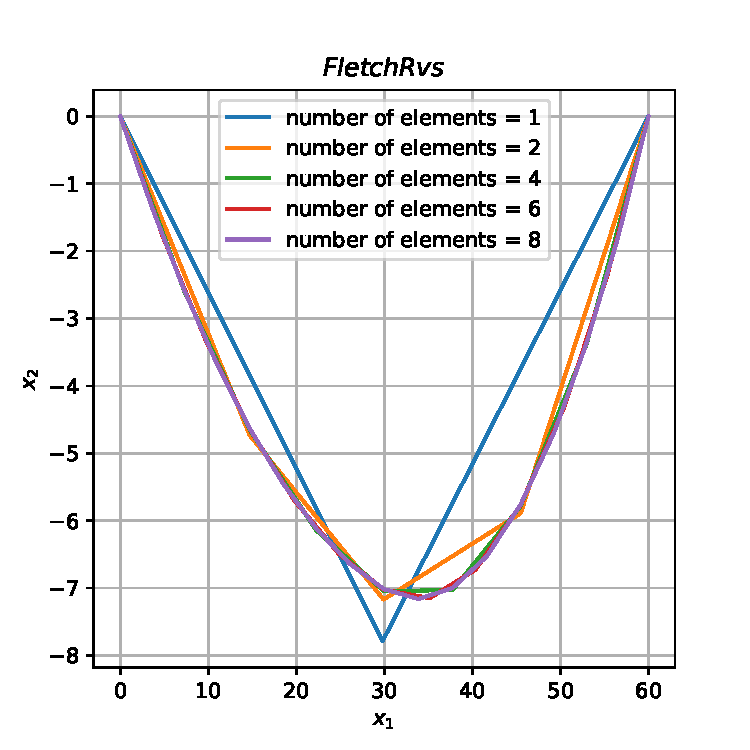
\includegraphics[width=\textwidth]{images/q2b_FletchRvs.pdf}
    \caption{Fletcher-Reeves}
    \label{fig:q2b_fletchrvs}
  \end{subfigure}
  \hfill
  \begin{subfigure}[b]{0.32\textwidth}
    \centering
    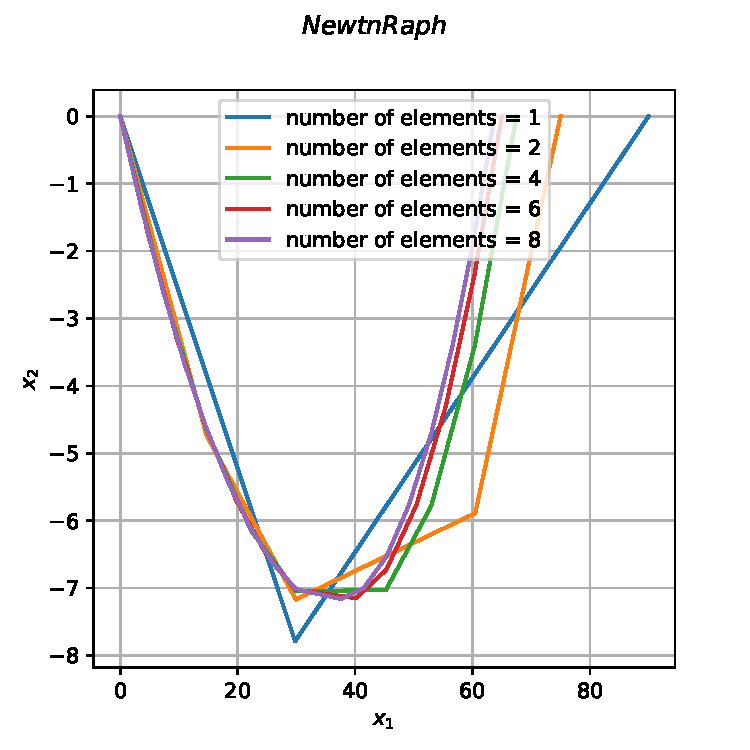
\includegraphics[width=\textwidth]{images/q2b_NewtnRaph.pdf}
    \caption{Newton-Raphson}
    \label{fig:q2b_newtnraph}
  \end{subfigure}
  \hfill
  \begin{subfigure}[b]{0.32\textwidth}
    \centering
    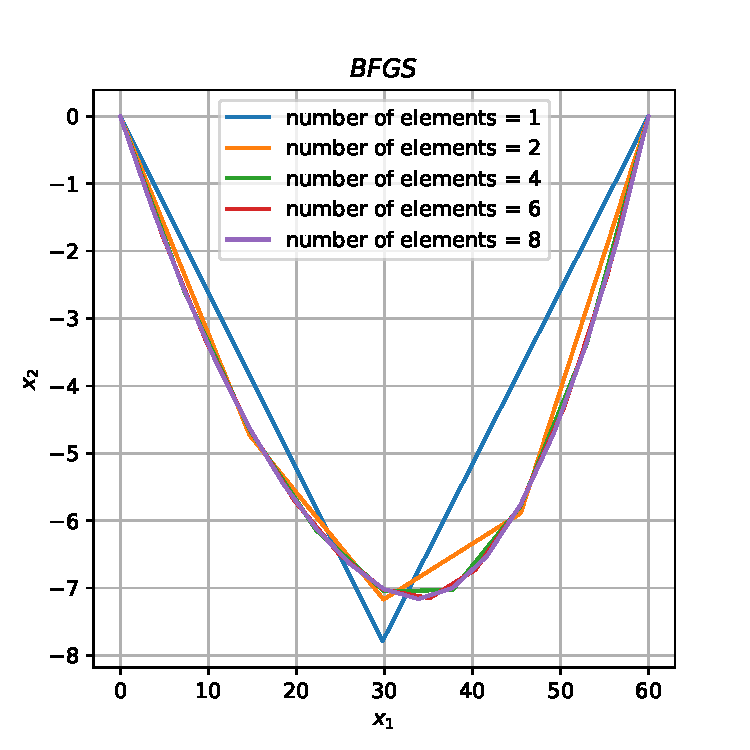
\includegraphics[width=\textwidth]{images/q2b_BFGS.pdf}
    \caption{BFGS}
    \label{fig:q2b_bfgs}
  \end{subfigure}
     \caption{Resultados da análise de convergência para discretizações maiores da mola}
     \label{fig:q2b}
\end{figure}

%%%%%%%%%%%%%%%%%%%%%%%%%%%%%%%%%%%%%%%%%%%%%%%%%%%

\bibliographystyle{apalike}
\bibliography{export}

\end{document}